\documentclass{kis}
%\addbibresource{references.bib}

\newacronym{pwm}{PWM}{Pulsbreitenmodulation}
\newacronym{uart}{UART}{Universal Asynchronous Receiver-Transmitter}
\newacronym{isr}{ISR}{Interrupt Service Routine}

%\newcommand{\todo}[1]{\textcolor{red}{TODO }\textcolor{red}{#1}}
\newcommand{\todo}[1]{\errmessage{Unresolved TODO: #1}}

\title{Laborbericht}

\begin{document}
\maketitle
\pagenumbering{Roman}
\setcounter{tocdepth}{2}
\tableofcontents
\listoffigures
\clearpage
\pagenumbering{arabic}

\section{Systemanalyse}

\subsection{Sensoren}
\subsubsection{Hallsonde} 
Eine Hallsonde (benannt nach ihrem Erfinder Edwin \textsc{Hall}) ist ein Sensor zur Messung von Magnetfeldern. Auch wenn solche Messinstrumente prinzipiell auch analoge Messungen durchführen können, wird er in dieser Anwendung ledglich als digitaler Sensor verwendet. An der Drehscheibe ist eine magnetische Markierung angebracht, wodurch eine an dem festen Aufbau angebrachte Hallsonde einen entsprechenden Logikpegel erzeugen kann. Diese Markierung ist so angebracht, dass an dem Digitalpin ein Low-Pegel anliegt, wenn sich das Loch der Drehscheibe über der Senke in dem Aufbau befindet. Die Hallsonde wird in diesem Aufbau also verwendet, um die Position des Lochs zu bestimmen. Wenn an dem Digitalpin der Hallsonde eine 1-0-Flanke detektiert wird, beginnt das Loch in der Drehscheibe sich mit dem Loch in der Senke zu überschneiden.

\subsubsection{Photosensor}
Auf der Unterseite der Drehscheibe befindet sich ein Muster ähnlich wie bei einem Glücksrad, aus sechs weißen und sechs schwarzen, jeweils alternierend Bereichen. Ferner befindet sich unter der Drehscheibe ein Photosensor, welcher verwendet werden kann, um die Farbe über diesem zu bestimmen. Auch hier ist der Sensor, obwohl er prinzipiell auch analog messen könnte, mit einem Digitalpin verbunden, sodass damit entsprechend der Farbe -- schwarz oder weiß -- einen High- oder Low-Pegel gemessen werden kann. Damit kann durch den Photosensor die Drehgeschwindigkeit der Scheibe gemessen werden. Aufgrund der Periodizität des ausgegeben Signals (siehe Abb. \ref{fig:photosensor}) kann aus dem Photosensor jedoch der aktuelle Drehwinkel nicht eindeutig bestimmt werden.

\begin{figure}
	\centering
	\input{photosensor.pdf_tex}
	\caption[Signal des Photosensors bei einer Umdrehung der Scheibe.]{Signal des Photosensors bei einer Umdrehung der Scheibe. Der Duty Cycle der periodischen Funktion beträgt genau $\frac{1}{2}$.}
	\label{fig:photosensor}
\end{figure}

Offensichtlich kann auch die Hallsonde die Drehgeschwindigkeit der Scheibe messen, doch der Photosensor ist für diese Aufgabe besser geeignet. Während die Hallsonde zur Bestimmung der Drehgeschwindigkeit mindestens eine volle Umdrehung benötigt, kann der Photosensor diese Messung in $\frac{1}{6}$ Umdrehung (wenn ein schwarz-weiß-Zyklus bestimmt wird) oder gar in nur $\frac{1}{12}$ Umdrehung (wenn nur ein schwarzes \emph{oder} ein weißes Feld verwendet wird) durchführen. Deshalb wäre bei Verwendung der Hallsonde zur Bestimmung der Drehgeschwindigkeit nur eine sehr langsame Reaktion auf sich ändernde Drehgeschwindigkeiten möglich.

Kurz zusammengefasst kann die Hallsonde sowohl die gewünschte Position als auch die Drehzahl bestimmen, während der Photosensor lediglich die Drehzahl bestimmen kann, für diese eine Aufgabe aber deutlich besser geeignet ist.

\clearpage
\subsection{Aktoren}
\subsubsection{Servoantrieb}
\begin{wrapfigure}[12]{r}{0.5\textwidth}
	\raggedleft
	\vspace*{-0.5\baselineskip}
	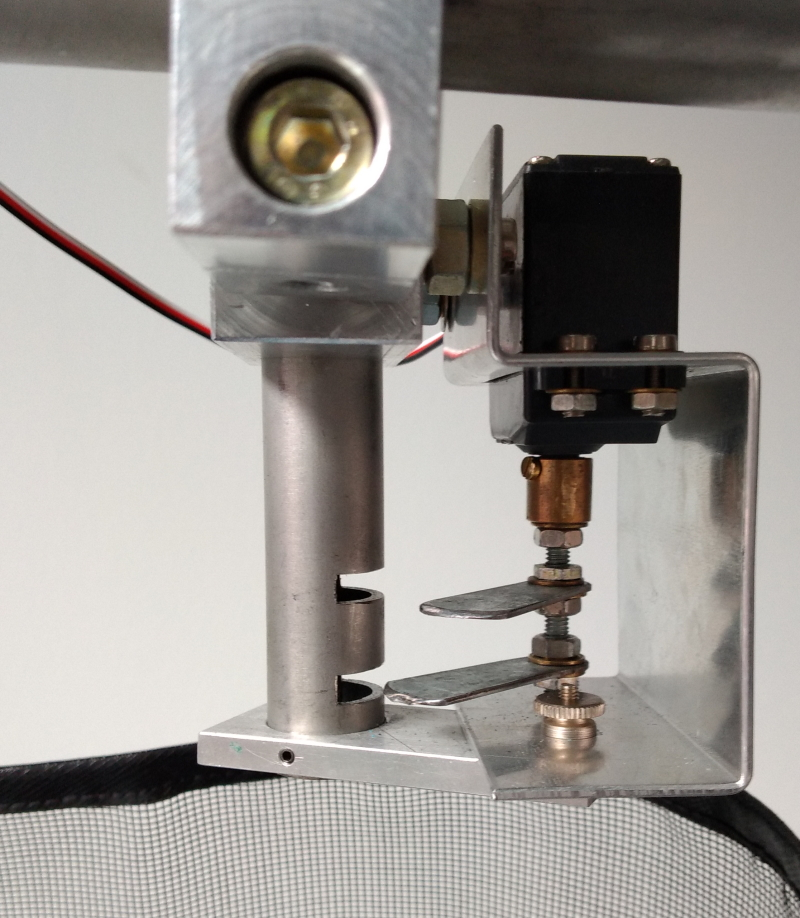
\includegraphics[width=0.9\linewidth]{IMG_20200525_171143701.jpg}
	\caption[Vorrichtung zum Abwurf der Kugeln]{Durch den Servoantrieb betriebene Vorrichtung zum Abwurf der Kugeln.}
\end{wrapfigure}
Bei einem Servoantrieb, wie er in dem Aufbau verwendet ist, erfolgt die Vorgabe der Sollgröße (d.h. des Winkels) üblicherweise über ein \gls{pwm}-Signal; durch eine interne Regelschleife wird der Servomotor auf die vorgegebene Position ausgeregelt. Da die Blackbox die Erzeugung des entsprechenden Signals nicht übernimmt, muss dies direkt durch den Arduino geschehen. Dafür existiert die \texttt{Servo}-Library, welche das \gls{pwm}-Signal für einen Winkel zwischen 0° und 180° erzeugt.
An der von dem Servoantrieb angetriebenen Welle befinden sich zwei versetzt angebrachte Zungen aus Metall, durch welche die Metallkugeln nacheinander freigesetzt werden können. Dabei sind zwei Stellungen von besonderer Wichtigkeit.

\begin{itemize}
\item[35°:] Hier blockiert die untere Zunge die unterste Kugel, die obere Zunge blockiert jedoch nichts, sodass eine oben eingeworfene Kugel in die Kammer fällt und dort verbleibt, bis die untere Zunge sie freigibt.
\item[60°:] Nun gibt die untere Zunge die Kammer frei, sodass die dort gelagerte Kugel herausfällt. Durch die Versetzung der beiden Zungen blockiert nun die obere Zunge die Kammer, sodass nur die eine in der Kammer befindliche Kugel freigesetzt wird und alle weiteren oben eingeworfenen Kugeln über der Kammer verbleiben.\\
Anmerkung: während des Semesters wurde der Aufbau offenbar leicht verändert. Zu Beginn der Systemanalyse lag der Winkel noch bei 50°. Andere Größen als die Verzögerung beim Abwurf der Kugel durch die Stellzeit des Servos wurden davon nicht beeinflusst.
\end{itemize}

Dies bedeutet, dass der Servoantrieb standardmäßig auf 35° gesetzt werden soll. Zur Freisetzung einer Kugel muss der Servoantrieb auf 60° ausgelenkt und anschließend wieder auf 35° gesetzt werden.

Eine mögliche Fehlerquelle, welche bereits bei der ersten Systemanalyse auffällt, ist die nichtvernachlässigbare Reaktionszeit der Abwurfvorrichtung aufgrund der langsamen Stellgeschwindigkeit des Servoantriebs. Dies hat eine höhere Zeitdifferenz zwischen (vermeintlichem) Abwurf und Auftreffen im Loch der Drehscheibe zur Folge, welche aber für alle Drehzahlen als konstant angenommen werden kann. Außerdem folgt daraus, dass die Zeit zum Auftreffen der Kugel experimentell bestimmt werden muss. Zwar kann die Fallzeit selbst aus den Gesetzen der Physik hergeleitet werden:
$$s(t) = \iint a(t) \text dt~\text dt\qquad\text{mit}~a(t) = \text{const.}$$
$$s(t) = \frac a2t^2+v_0t+s_0\qquad\text{mit}~v_0=0;~ s_0=0$$
\begin{align*}t_\text{Fall} &= \sqrt{\frac{2s}{a}}\qquad \text{mit}~s=0,72~\text{m};~ a=g=9,81~\frac{\text{m}}{\text{s}^2}\\
&= \sqrt{\frac{2\cdot0,72~\text{m}}{9,81~\frac{\text{m}}{\text{s}^2}}}\\
&= 0,383~\text{s}\end{align*}
Diese Zeit würde jedoch nicht die nicht vernachlässigbare Stellzeit des Servoantriebs einschließen. Diese muss experimentell bestimmt werden. Dabei ergab sich:
\begin{align*}t &= t_\text{Stell} + t_\text{Fall}\\
&= 0,495~\text{s}\end{align*}

\newpage
\subsection{Kommunikation mit dem Nutzer}

\subsubsection{Serielle Schnittstelle}
Das Arduino-Board kommuniziert über eine serielle USB-\gls{uart}-Schnittstelle mit dem PC. Dadurch können durch eine entsprechend konfigurierte Software auf dem PC Daten vom Arduino empfangen und zum Arduino gesendet werden.

\subsubsection{Trigger}
Über ein Kabel ist ein kleines Bediengerät mit der Blackbox verbunden, welches einen Knopf besitzt. Wenn der Knopf darauf gedrückt wird, liegt an dem entsprechenden Pin ein High-Pegel an; ansonsten ein Low-Pegel. Dieses Bediengerät kann sehr gut zum Start der Durchführung verwendet werden. 

\subsubsection{Sonstiges}
\paragraph{Buttons}
Es gibt zwei Buttons auf dem Arduino-Board. Durch diese wird erwartungsgemäß ein High-Pegel an dem entsprechenden Pin angelegt, wenn sie gedrückt werden, und ansonsten ein Low-Pegel.
\paragraph{Kippschalter}
Der auf der Blackbox angebrachte Kippschalter legt in der unteren Stellung (\glqq Controller\grqq) einen High-Pegel an dem Pin an; in der oberen Stellung (\glqq Direct\grqq) sowie in der Zwischenstellung einen Low-Pegel.
\paragraph{LEDs}
Von den beiden LEDs auf dem Daughterboard, das oben auf dem Arduino-Board angebracht ist, leuchtet LED 1 gelb, LED 2 leuchtet grün. An der Blackbox ist ebenfalls eine ansteuerbare LED angebracht. Bei einem angelegten High-Pegel leuchten die LEDs jeweils, bei einem Low-Pegel bleiben sie aus. Der Pin der LED 2 ist außerdem mit der onboard-LED des Arduino-Boards verbunden.

Die LEDs auf dem Daughterboard werden verwendet, um die aktuelle Drehgeschwindigkeit als Ampel anzuzeigen -- bei langsamer Drehgeschwindigkeit ist die grüne LED an, bei mittelschneller Drehgeschwindigkeit beide und bei schneller Umdrehung nur die gelbe LED. Die LED an der Blackbox wird verwendet, um unerwartetes, d.h. nicht bloß durch Reibung verursachtes Abbremsen oder Beschleunigen der Scheibe anzuzeigen.

\subsection{Machbarkeitsanalyse}
\subsubsection{Ungenauigkeit der Abwurfvorrichtung}
Die Machbarkeitsanalyse hat einige Probleme des Aufbaus aufzeigen können. Das auffälligste Problem ist ein sehr großer und leicht versetzter Fallradius der Kugeln.

Bei ein Test mit manuellem Auslösen der Kugeln mit Hilfe des Triggers trafen selbst \emph{bei Stillstand der Scheibe} nicht alle Kugeln zuverlässig das Loch. Selbst bei Stillstand der Scheibe verfehlten zwischen $\frac13$ und $\frac12$ der abgeworfenen Kugeln die Senke und prallten an dem äußeren Rand des Lochs in der Scheibe ab.

Dieses Verhalten ist einzig und allein dem physikalischen Aufbau des Systems geschuldet. Die Software wird nicht in der Lage sein, die Unzulänglichkeiten des Aufbaus zu korrigieren, wodurch bereits bei ersten, einfachen Tests des Aufbaus berechtigte Zweifel an der Machbarkeit aufkommen.

Der Versuchsaufbau besitzt folgende Probleme, welche Grund für dieses Verhalten sein können.
\begin{itemize}
	\item Der Aufbau steht nicht perfekt gerade, sondern ist um einen geringen Winkel geneigt, wodurch die Kugel weiter außen auftrifft als erwartet.
	\item Die Lagerung der Scheibe besitzt relativ viel Spiel, sodass sich die Scheibe unrund dreht.
	\item Das Loch in der Scheibe ist nicht perfekt konzentrisch.
	\item Das Rohr in der Abwurfvorrichtung, durch welche die Kugeln fallen, besitzt ein Übermaß, sodass nicht gewährleistet werden kann, dass die Kugel mittig durch die Vorrichtung fällt.
\end{itemize}
Des weiteren kann die Kugel durch den Auslösemechanismus einen leichten Drall erhalten. Dessen Einfluss ist jedoch vernachlässigbar -- damit dieser Effekt einen nennenswerten Einfluss bekommt, müsste der Servoantrieb deutlich schneller sein. Außerdem kann durch einen gezielten Drall, selbst wenn dieser einen nennenswerten Einfluss hätte, die Kugel nur in eine Richtung gelenkt werden. Es zeigt sich jedoch, dass aufgrund des es Übermaßes der Abwurfvorrichtung und dem daraus resultierenden Spiel der Kugel im Rohr, die Kugel das Loch an beiden Seiten verfehlen kann. Ein gezielter Drall kann dieses Problem nicht beheben.

Diese Streuung der Kugeln findet im nicht nur in radiale, sondern auch in tangentiale Richtung der Scheibe, wenngleich die Streuung in tangentiale Richtung nicht so stark ist, statt. Das ist insoweit problematisch, als dass rechtzeitig abgeworfene Kugeln so fälschlicherweise verfrüht oder verspätet wirken.

%\todo{Machbarkeit der Signal-Verzögerung der Sensoren}

\subsubsection{Machbarkeit der Abbremsungsbestimmung}
Es ist möglich, unerwartete Abbremsungen und Beschleunigungen der Scheibe zu bestimmen; unter Umständen kann darauf jedoch nicht schnell genug reagiert werden, sodass die nächste abzuwerfende Kugel das Ziel trotzdem verfehlt. Dies wird dann auftreten, wenn die Außeneinwirkung zwischen dem Referenzpunkt der Hallsonde und dem Auslösen des Abwurfmechanismus auftritt. In diesem Fall wird die nächste -- und nur die nächste -- Kugel das Ziel verfehlen. Auf Abbremsungen zu anderen Zeitpunkten sollte jedoch ohne Probleme reagiert werden können. Im schlimmsten Fall wird bei einer Abbremsung oder Beschleunigung durch Außeneinwirkung also höchstens eine Kugel das Ziel verfehlen.

\subsubsection{Fazit zur Machbarkeit}
Aufgrund der Unzulänglichkeiten im Aufbau, welche durch die Software nicht korrigierbar sind, kann kein zuverlässiges System entstehen. Es kann aber gezeigt werden, dass die Software funktioniert und die Kugeln treffen würden, wenn der Abwurf der Kugeln ausreichend genau wäre.

\section{Design}
\subsection{Wahl der Randbedingungen}
\paragraph{Drehgeschwindigkeit}
Es werden folgende Schwellwerte für die Drehgeschwindigkeit festgelegt:
\begin{itemize}
	\item Langsam: $t_r>3~\text{s/U}$
	\item Mittelschnell : $1~\text{s/U}\leq t_r\leq 3~\text{s/U}$
	\item Schnell: $t_r<1~\text{s/U}$
\end{itemize}

\paragraph{Aufbau}
Es wurde der Aufbau im Raum Z 2045 gewählt. Die Scheibe wird entgegen dem Uhrzeigersinn gedreht.

\subsection{Grobentwurf}
Der Entwurf sowie die Implementierung werden Anhand des in Abb. \ref{fig:lösungsstack} gezeigten Lösungsstacks durchgeführt, wobei der Hardwarelayer bereits durch den Kugelfall-Aufbau, die Blackbox und das Arduino-Shield gegeben ist. Der hardwarenahe Softwarelayer soll einige wichtige Funktionen des Aufbaus gegenüber dem Anwendungslayer abstrahieren, während der Anwendungslayer den Algorithmus zum spezifikationsgerechten Abwurf der Kugeln bereitstellt.

\begin{figure}
	\centering
	\newcolumntype{Y}{>{\centering\arraybackslash}X}
	\renewcommand{\arraystretch}{1.7}
	\begin{tabularx}{0.8\textwidth}{|Y|}
		\hline
		\large Anwendungslayer\\
		\small \texttt{algorithm.ino} -- Algorithmus zum Abwurf der Kugeln\\
		\hline
		\large Hardwarenaher Softwarelayer\\
		\small \texttt{kugelfall\_interrupt.h} -- Funktionen zur Abstraktion der Hardware\\
		\hline
		\large Hardwarelayer\\
		\small Blackbox -- Verbindung zum Testaufbau selbst\\
		\hline
	\end{tabularx}
	\caption{Lösungsstack.}
	\label{fig:lösungsstack}
\end{figure}

\subsection{Hardwareanbindung}
Konkret bestehen die Aufgaben des hardwarenahen Softwarelayers aus folgendem:

\paragraph{Exakte Messungen mittels Interrupts}
Das erste Design sah eine Lösung mittels Polling bei Bedarf vor, die aber nach genauerer Betrachtung verworfen wurde. Der Arduino stellt Interrupts für die Pins des Photo- und Hallsensors zur Verfügung. Diese werden ausgeführt, wenn eine steigende Flanke am Pin des Photosensors bzw. eine fallende Flanke am Pin des Hallsensors bemerkt wird. Interrupts bieten eine exaktere Zeitbestimmung als Polling oder das Abfragen von Pins im Anwendungslayer. Die Messwerte, die in einer \gls{isr} ermittelt werden, werden in globalen, als \texttt{volatile} gekennzeichneten Variablen gespeichert und zur Verfügung gestellt.

\paragraph{Bestimmung der Drehgeschwindigkeit der Scheibe}
Für diese Aufgabe wird gemäß der Vorbetrachtung der Photosensor verwendet. Durch Messung der für einen schwarz-weiß-Zyklus benötigten Zeit und Multiplikation mit dem Faktor 6 kann die Zeit für eine volle Umdrehung bestimmt werden. Diese Messung war zunächst als normale Funktion geplant, wurde später aber durch Interrupts vereinfacht. Die \gls{isr}, die in der finalen Implementierung verwendet wird, stellt für den Photosensor den letzten und den aktuellen Zeitpunkt einer 0-1-Flanke, also das Ende eines schwarz-weiß-Zyklus zur Verfügung. Aus der Geschwindigkeit wird außerdem die Kategorie (langsam, mittelschnell, schnell) berechnet und wie bereits erklärt durch LEDs angezeigt. Gespeichert werden jeweils die Geschwindigkeit der letzten und der aktuellen Umdrehung.

\paragraph{Abbremsungsbestimmung}
In der Designphase sollte die Abbremsung bestimmt werden, indem zwei oder mehr schwarz-weiß-Zyklen des Photosensors beobachtet und ihre Geschwindigkeiten verglichen werden. Zwei Zyklen sind allerdings nicht ausreichend genau, worauf im Kapitel zur Implementierung genauer eingegangen wird. Im finalen Design ruft die ISR des Photosensors nach der Geschwindigkeitsbestimmung mit einem Zyklus eine Funktion auf, die die gemessene Geschwindigkeit mit der Geschwindigkeit der letzten Umdrehung vergleicht und bestimmt, ob die Abbremsung für den physikalischen Aufbau normal ist, oder ein aktives Abbremsen vermutet werden kann.

\paragraph{Bestimmung der Position des Lochs}
Die Position des Lochs kann auf zwei Arten bestimmt werden. Der hardwarenahe Softwarelayer stellt einmal eine Warte-Funktion zur Verfügung, welche die Ausführung des Programms so lange blockiert, bis an dem Digitalpin der Hallsonde die zuvor erläuterte 1-0-Flanke beginnt. Die Entscheidung, wann die Kugel auf Grundlage dessen abgeworfen werden soll, obliegt anschließend dem Anwendungslayer. Die zweite Funktion, die nach der Designphase dazu gekommen ist, ist eine \gls{isr}, die durch eine 1-0-Flanke des Hallsensors ausgelöst wird. Diese ISR berechnet aus dem aktuellen Zeitpunkt der Flanke den erwarteten nächsten Zeitpunkt einer 1-0-Flanke mit Hilfe der aktuellen Drehgeschwindigkeit. Sowohl der aktuelle als auch der vorhergesagte Zeitpunkt der 1-0-Flanke werden gespeichert.

\paragraph{Bereitgestellte Messwerte}
Zusammenfassend bildet das mittlere Layer die Schnittstelle zwischen Hardware und Software, indem es folgende Messwerte zur Verfügung stellt: Die letzte 0-1-Flanke des Photosensors, die Drehgeschwindigkeit in der letzten Umdrehung und in der aktuellen Umdrehung, die letzte 1-0-Flanke des Hallsesnsors und die berechnete erwartete nächste 1-0-Flanke, den Geschwindigkeitsmodus (langsam, mittel, schnell) angezeigt durch die gelbe und grüne LED und ein Flag für unvorhergesehene Abbremsung der Scheibe angezeigt durch die LED auf der Blackbox.


\subsection{Algorithmus zum Abwurf der Kugeln}

Der Algorithmus ist seit dem ersten Design stark vereinfacht worden, da das Abfragen der Sensoren durch Polling nicht mehr beachtet werden muss. Der in diesem Abschnitt beschriebene Polling-Ansatz ist in der finalen Implementierung nicht mehr vorhanden. Der erste Entwurf sah folgendes vor:

\paragraph{Repräsentation des Abwurf-Musters}
Der Algorithmus zum Abwurf der Kugeln findet in dem Main Loop des Hauptprogramms statt. Die Schleife wird solange durchlaufen, bis das Drücken des Knopfes auf dem Steuergerät als Trigger erkannt wird. Abhängig vom Geschwindigkeitsmodus werden verschiedene Muster aus Kugel Abwerfen und Umdrehungen auslassen ausgeführt. Damit nicht für jeden Geschwindigkeitsmodus eine andere Schleife notwendig ist, sind die Muster in einem Array hinterlegt mit einer Zeile für jeden Geschwindigkeitsmodus. 

\paragraph{Prüfen der Geschwindigkeit}
Vor der Ausführung des Musters wird zunächst geprüft, ob der Geschwindigkeitsmodus noch der selbe ist. Falls nicht, wird ein Hinweis ausgegeben, das Muster aber fortgesetzt. Außerdem wird die aktuelle Geschwindigkeit der Scheibe auf unvorhergesehene Abbremsung geprüft. Dafür wird im ersten Entwurf eine Funktion aufgerufen, die returnt, wenn die Geschwindigkeit valide ist und sonst darauf wartet, dass die Geschwindigkeit vorhersagbar wird bevor sie returnt.

\paragraph{Abwerfen der Kugel}
Zunächst wird die Wartezeit berechnet, bis die Kugel abgeworfen werden soll. Dazu wird die Differenz aus dem erwarteten nächsten Zeitpunkt, an dem das Loch der Scheibe unter der Kugel sein wird, der experimentell bestimmten Verzögerung bis zum Auftreffen der Kugel und der aktuellen Zeit bestimmt. Während auf das Öffnen des Servo gewartet wird, muss auch bemerkt werden, wenn sich der Wert des Hallsensor Pins ändert, um die Position des Lochs für die folgenden Runden korrekt zu bestimmen. Bevor der Befehl zum Schließen des Servos gegeben wird, wird ebenfalls gewartet, damit sicher gestellt ist, dass sich der Servo ganz geöffnet hat. In der Zwischenzeit wird eine Geschwindigkeitsmessung durchgeführt. Auch in der Zeit muss auf den Hallsensor gehört werden.

\paragraph{Auslassen einer Umdrehung}
Es wird auf eine 1-0-Flanke des Hallsensors gewartet.

\paragraph{Muster beendet}
Es wird mit der Abbruchbedingung \texttt{patternDone = true;} die Schleife verlassen, so dass das Main Loop wieder auf Auslösen des Triggers wartet.

\paragraph{Overhead durch Polling}
Im ersten Design des Algorithmus waren die benötigten Messwerte jedoch nicht automatisch durch den hardwarenahen Layer verfügbar. Deshalb wurde die Geschwindigkeit der Scheibe zwischen Öffnen und schließen des Servos gemessen. Zwischen Öffnen und Schließen des Servos muss sowieso gewartet werden, damit der Servo vollständig geöffnet ist. Einen vollständigen schwarz-weiß-Zyklus abzuwarten dauert den angefangenen Zyklus und den nächsten Zyklus, der gemessen werden soll, also mindestens eine Drittel Umdrehung der Scheibe. Ohne unnatürliche Beschleunigung der Scheibe reicht diese Zeit aus, um den nächsten Abwurfzeitpunkt nicht zu verpassen. Allerdings muss während der Geschwindigkeitsmessung auch auf den Hallsensor gehört werden, da die Position des Lochs in diesem Zeitraum liegen kann. Dadurch wird die Funktion zur Geschwindigkeitsmessung unnötig komplex. Auf den Hallsensor muss auch beim Warten auf den Abwurfzeitpunkt gehört werden. Deshalb wurde die \texttt{delay()} Funktion im ersten Entwurf vollständig durch eine Schleife \texttt{while(millis() < abwurf)} ersetzt, die in jedem Durchlauf auf Änderung der Sensoren testet. Dennoch wurden 1-0-Flanken des Hallsensors verpasst, so dass der vorhergesagte Zeitpunkt auch für die nächste Vorhersage verwendet werden musste und sich Fehler addiert haben. Der Interrupt-Ansatz in der Implementierung ist daher deutlich präziser.

\section{Implementierung}

\subsection{Implementierung des Entwurfs}
\subsubsection{Hardwareanbindung}
In der Embedded-Programmierung gilt es immer, ein sinnvolles Gleichgewicht zwischen Abstraktion und Performanz zu finden. Bei 32~kB Flash-Speicher und nur 2~kB RAM kann sich überflüssige Objektorientierung, wenngleich sie unbestreitbar die Lesbarkeit des Codes verbessert, eher kontraproduktiv auswirken.

Um die zugrundeliegende Hardware zu abstrahieren, wird eine Header-Datei erstellt, welche einige Funktionen und Struts bereitstellt und von dem Anwendungslayer eingebunden werden kann. Dieser Ansatz entspricht auch im Wesentlichen dem Industriestandard bei Embedded-Software.

\paragraph{Vorbereitung der Hardware}
Die Pinbelegung wird ebenfalls in der Header-Datei spezifiziert. Die Funktion \texttt{setupHardware()} initialisiert die Pins und legt die Baudrate für die serielle Schnittstelle fest.

\paragraph{Messung der Drehung der Scheibe}
Anfangs war geplant, die Drehung der Scheibe Polling-basiert zu erhalten. Dabei mussten jedoch sehr viele Randfälle beachtet werden, z.B. \glqq{}Was passiert, wenn während der Geschwindigkeitsmessung die 1-0-Flanke auf der Hallsonde stattfindet?\grqq{}. Bei dem Arduino Uno ist es möglich die Pins 2 und 3, welche praktischerweise mit Hallsonde und Photosensor verbunden sind, als Interruptpins zu verwenden und diese mit einer \gls{isr} zu assoziieren. Indem der letzte Aufrufzeitpunkt der \gls{isr} in einer geteilten Variable gespeichert wird, kann so mit jedem Aufruf der \gls{isr} die aktuelle Drehgeschwindigkeit upgedated werden. 

\iffalse
Es ist nicht besonders sinnvoll, zwei separate Funktionen zur Messung der Drehgeschwindigkeit und zur Messung der Abbremsung zu haben -- wenn die Abbremsung gemessen werden soll, muss dazu die Drehgeschwindigkeit ebenfalls gemessen werden. Um dies zu realisieren, existiert die \texttt{rotationMeasure()}-Funktion, welche über eine als Argument zu übergebende Anzahl schwarz-weiß-Zyklen (wenigstens zwei) die Drehgeschwindigkeit und die Abbremsung der Scheibe misst und einen Struct mit den Attributen \texttt{time} (Einheit: ms/U) und \texttt{deceleration} (Einheit: ms/U$^2$) zurückgibt.

Die Funktion ist als Pseudocode in Abbildung \ref{fig:pseudo-dreh} gezeigt.

Diese Funktion sorgt außerdem dafür, die LEDs entsprechend der gemessenen Drehgeschwindigkeit ein- und auszuschalten. Bei langsamer Drehung leuchtet die grüne LED, bei mittelschneller Drehung leuchten beide LEDs und bei schneller Drehung leuchtet nur die orangene LED.

\begin{figure}[H]
\lstset{basicstyle=\small\ttfamily,tabsize=4}
{\singlespacing
\begin{lstlisting}[frame=single]
function measureRotation() => integer, integer

	# sicherstellen, dass Messung nicht mitten auf Feld beginnt
	while read(PhotoSensorPin) = 1 loop
		idle
	end while
	while read(PhotoSensorPin) = 0 loop
		idle
	end while

	# zwei 1-0-Zyklen messen
	tBeforeFirstCyc := millis()

	for i from 0 to 2 loop
		while read(PhotoSensorPin) = 1 loop
			idle
		end while
		while read(PhotoSensorPin) = 0 loop
			idle
		end while
		
		if i = 1 then
			tAfterFirstCyc := millis()
		end if
	end for	
	
	tAfterSecondCyc := millis()
	
	t_r1 := 6 * (tAfterFirstCyc - tBeforeFirstCyc)
	t_r2 := 6 * (tAfterSecondCyc - tAfterFirstCyc)
	
	t_r := (t_r1 + t_r2) / 2
	delta_t_r := (t_r2 - t_r1)
	
	return t_r, delta_t_r
	
end function
\end{lstlisting}
}
\caption{Pseudocode zur Bestimmung der Drehgeschwindigkeit.}
\label{fig:pseudo-dreh}
\end{figure}
\fi

\paragraph{Bestimmung der Position des Lochs}
Die Funktion \texttt{awaitHallSensorPosition()} wartet auf die nächste 1-0-Flanke des Pins der Hallsonde und blockiert die Ausführung des Programms währenddessen. Dadurch kann synchron auf die Position des Lochs gewartet werden. Bei der Ausführung ist jedoch ein asynchroner Ansatz wünschenswerter, weshalb außerdem eine \gls{isr} existiert, welche den aktuellen Zeitstempel in Millisekunden in eine geteilte Variable speichert, welche dann vom Anwendungslayer verrechnet werden kann.

\begin{figure}
\lstset{basicstyle=\small\ttfamily,tabsize=3}
{\singlespacing
\begin{lstlisting}[frame=single]
function awaitHallSensorPosition()

	# Anfang eines High-Pegels erwarten
	while read(HallSensorPin) = 0 loop
		idle
	end while
	
	# Ende des High-Pegels erwarten
	while read(HallSensorPin) = 1 loop
		idle
	end while
	
	# Prozessor freigeben sobald der High-Pegel vorbei ist
	return
	
end function
\end{lstlisting}
}
\caption{Pseudocode zur Bestimmung der Position des Lochs.}
\label{fig:pseudo-loch}
\end{figure}

\paragraph{Überprüfung der Implementierung}
In den Abbildungen \ref{fig:turn_time} bis \ref{fig:deceleration_true} ist kurz der zeitliche Verlauf der Drehzeit $t_r$ sowie der Abbremsung der Scheibe dargestellt. Dabei zeigte sich, dass der angenommene, lineare Verlauf der Drehgeschwindigkeit nicht immer Gültigkeit besitzt. Bei sehr niedrigen Drehgeschwindigkeiten kann der richtigerweise als exponentialförmig vorhergesagte Verlauf nicht mehr mit ausreichender Genauigkeit linearisiert werden.

Außerdem ist die Berechnung der Abbremsung aus zwei Zyklen mit anschließender Extrapolation nicht ausreichend genau ist.

Die quantitativen Unterschiede zwischen Abb. \ref{fig:deceleration_five} und den anderen drei Abbildungen sind auf einen etwas anderen Beginn der Messung (die Scheibe wurde bei diesem Durchlauf nicht genau mit derselben Anfangsgeschwindigkeit angestoßen) zurückzuführen.

\clearpage
\begin{figure}
	\input{turn_time_two_cycles.pdf_tex}
	\caption[Verlauf der Drehzeit der Scheibe.]{Verlauf der Drehzeit der Scheibe nachdem das System angestoßen wurde.}
	\label{fig:turn_time}
\end{figure}

\begin{figure}
	\input{decleration_two_cycles.pdf_tex}
	\caption[Über zwei Zyklen gemessene und extrapolierte Abbremsung der Scheibe]{Über zwei Zyklen gemessene und extrapolierte Abbremsung der Scheibe nachdem das System angestoßen wurde. Man beachte die durch die Extrapolation aus einem zu kurzen Intervall verstärkten Messfehler (negative Abbremsung) sowie die generell zu geringe Abbremsung.}
	\label{fig:deceleration_two}
\end{figure}

\begin{figure}
	\input{decleration_five_cycles.pdf_tex}
	\caption[Über fünf Zyklen gemessene und extrapolierte Abbremsung der Scheibe.]{Über fünf Zyklen gemessene und extrapolierte Abbremsung der Scheibe nachdem das System angestoßen wurde. Der Verlauf ist deutlich sauberer und stimmt auch quantitativ mit dem zeitlichen Verlauf aus Abb. \ref{fig:turn_time} und \ref{fig:deceleration_true} überein.}
	\label{fig:deceleration_five}
\end{figure}

\begin{figure}
	\input{true_decleration_two_cycles.pdf_tex}
	\caption{Echte, aus der Drehzeit berechnete Abbremsung der Scheibe nachdem das System angestoßen wurde.}
	\label{fig:deceleration_true}
\end{figure}
\clearpage

\subsubsection{Algorithmus zum Abwurf der Kugeln}
\paragraph{Repräsentation des Abwurf-Musters}
Der Algorithmus zum Abwurf der Kugeln findet in dem Main Loop des Hauptprogramms statt. Die Loop wird solange durchlaufen, bis das Drücken des Knopfes auf dem Steuergerät als Trigger erkannt wird. Abhängig vom Geschwindigkeitsmodus werden verschiedene Muster aus Kugel Abwerfen und Umdrehungen auslassen ausgeführt. Damit nicht für jeden Geschwindigkeitsmodus eine andere Schleife notwendig ist, sind die Muster in einem Array hinterlegt, das wie folgt aufgebaut ist. 
$$\texttt{throwMarble[veloMode][turn]} = 
\left( \begin{array}{rrrrrrrrrr} 
 1 &  0 &  1 &  0 &  1 & -1 & -1 & -1 & -1 & -1 \\
 1 &  0 &  1 &  1 &  0 &  0 &  1 &  1 &  1 & -1 \\
 1 &  1 &  1 & -1 & -1 & -1 & -1 & -1 & -1 & -1 \\ 
\end{array} \right)$$
Die Zeilen stehen für die unterschiedlichen Geschwindigkeitsmodi, dabei steht 0 (oben) für schnell, 1 für mittlere Geschwindigkeit und 2 für langsam. Die Spalten präsentieren die Umdrehungen seit Beginn des Abwurf-Musters. Hier steht die erste Spalte für die erste Kugel und aufsteigende Werte für die folgenden Umdrehungen der Scheibe. Die Einträge der Matrix sind 1 für das Abwerfen der Kugel, 0 für das Auslassen einer Umdrehung und -1 als Signal, dass das Muster fertig abgearbeitet ist, da die Muster unterschiedlich lang sind.
Beim Auslösen des Triggers wird dann anhand des Geschwindigkeitsmodus die richtige Zeile der Matrix ausgewählt und ausgeführt bis eine -1 gelesen wird. Danach wird wieder auf den Trigger gewartet. Im Detail passiert bei jeder Umdrehung folgendes:

\paragraph{Prüfen der Geschwindigkeit}
Vor der Ausführung des Musters wird zunächst geprüft, ob der Geschwindigkeitsmodus noch der selbe ist. Falls nicht, wird ein Hinweis ausgegeben, das Muster aber fortgesetzt. Außerdem wird die aktuelle Geschwindigkeit der Scheibe auf unvorhergesehene Abbremsung geprüft. Dazu wird eine Flag verwendet, die vom hardwarenahen Layer zur Verfügung gestellt wird und unerwartet starkes Abbremsen anzeigt. Ist das der Fall, wird mit die Ausführung des Musters pausiert bis die Abbremsung wieder den normalen physikalischen Gegebenheiten entspricht, jedoch mindestens eine ganze Umdrehung.

\paragraph{Abwerfen der Kugel}
Zunächst wird die Wartezeit berechnet, bis die Kugel abgeworfen werden soll. Dazu wird die Differenz aus dem erwarteten nächsten Zeitpunkt, an dem das Loch der Scheibe unter der Kugel sein wird und der aktuellen Zeit bestimmt. Zudem wird die oben beschriebene experimentell bestimmte Zeit zum Auslösen des Servos und die Fallzeit der Kugel abgezogen, hier beides zusammengefasst in \texttt{fallTime}.
$$\texttt{int t = expHallFlip - millis() - fallTime;}$$
Es kann passieren, dass einmal beim Auslösen des Triggers in der ersten Umdrehung der Abwurfzeitpunkt für diese Umdrehung schon verstrichen ist, also $t < 0$. In dem Fall wird eine auf die nächste Runde gewartet, indem die aktuell gemessene Zeit für eine Umdrehung zu $t$ addiert wird.
$$\texttt{t = t + currentTurnTime;}$$
Es wird für die berechnete Zeit $t$ gewartet bis der Servo geöffnet und eine Kugel abgeworfen wird. Bevor der Befehl zum Schließen des Servos gegeben wird, wird ebenfalls gewartet. Die Wartezeit ist das Minimum aus 500~ms oder einer halben Umdrehung, um sicher zu stellen, dass der Servo zuvor komplett geöffnet war.

\paragraph{Auslassen einer Umdrehung}
Es wird für die aktuell gemessene Zeit einer Umdrehung gewartet.

\paragraph{Muster beendet}
Es wird mit der Abbruchbedingung \texttt{patternDone = true;} die Schleife verlassen, so dass das Main Loop wieder auf Auslösen des Triggers wartet.


\subsubsection{Bestimmung unerwarteter Drehgeschwindigkeiten}
Um unerwartete Drehgeschwindigkeiten zu detektieren, muss natürlich die erwartete Drehgeschwindigkeit, bzw. die erwartete Abbremsung unter Abhängigkeit der aktuellen Drehgeschwindigkeit bestimmt werden. Diese wird als stückweise stetige Funktion approximiert.
$$\Delta t_{ok} = \begin{cases}
    20, & \phantom{0000 <} t \leq 900\\
    \frac{t-900}{20} + 20, & \phantom{0}900 < t \leq 2200\\
    \frac{t-2200}{10} + 85, & 2200 < t \leq 2500\\
    \infty, & 2500 < t
\end{cases}$$
Die Abbremsung $\Delta t$ wird akzeptiert, wenn $\Delta t < \Delta t_{ok}$ ist. Für $t>2500$ ist die Abbremsung durch Reibung so groß, dass menschengemachte Abbremsung nicht mehr zuverlässig gemessen werden kann. In dem Fall werden alle $\Delta t$ akzeptiert.

In Abb. \ref{fig:acceptable_deceleration} sind echte Abbremsung und stückweise defininerte Funktion gegenüber gestellt.

\begin{figure}
	\input{acceptable_deceleration.pdf_tex}
	\caption[Akzeptierte Abbremsung der Scheibe.]{Akzeptierte Abbremsung und Abbremsung ohne Fremdeinwirkung in Abhängigkeit der Zeit $t_r$ für eine Umdrehung. Wenn die gemessene Abbremsung über der akzeptierten Abbremsung liegt, wird von Fremdeinwirkung ausgegangen.}
	\label{fig:acceptable_deceleration}
\end{figure}

%\vfill
%\fbox{\begin{minipage}{\textwidth}
%Im abgegebenen Code ist \texttt{algorithm.ino} und \texttt{kugelfall.h} die Polling-basierte Lösung, während \texttt{algorithm2.ino} und \texttt{kugelfall\_interrupt.h} die Interrupt-basierte Lösung darstellt. Es soll bitte nur letztere in die Bewertung eingehen.
%\end{minipage}}
%\vfill

\subsection{Umstieg auf eine Interrupt-basierte Lösung}
Nachdem sehr viel -- zu viel -- Zeit damit verschwendet wurde, bei der anfangs geplanten Polling-basierten Lösung alle Randfälle beim Polling abzufangen, wodurch sehr unschöner und verschlungener Spaghetticode entstand, wurde dieser Ansatz verworfen und auf eine Interrupt-basierte Lösung zur Aufnahme der Sensorwerte übergegangen. Dieser Ansatz ist deutlich eleganter, für die beiden Sensoren existiert jeweils ein Interruptpin, welcher mit einer entsprechenden \gls{isr} assoziiert wird. Dies erlaubt es, die Aufnahme der Messdaten und die Durchführung des Algorithmus zum Abwurf der Kugeln pseudo-gleichzeitig durchzuführen, während bei dem Polling-basierten Ansatz immer zwischen Messdatenaufnahme und Algorithmus hin-und-her gewechselt werden musste.

Während im Entwurf größtenteils der Polling-Ansatz erläutert wurde, da dieser auch die längste Zeit geplant war, bezieht sich das Kapitel zur Implementierung auf den Interrupt-Ansatz.

Nachdem der Interrupt-Ansatz verwendet wurde, konnte das Programm von dem vorherigen Spaghetticode befreit werden. Auch die gewünschte Trennung zwischen Hardwareanbindung und Algorithmus konnte so deutlich besser gewährleistet werden.

\subsection{Fehlerfindung und -behebung}

\subsubsection{Auslassen einer Umdrehung nach dem Abwurf einer Kugel}
\paragraph{Symptom}
Nachdem sichergestellt werden konnte, dass die Kugeln zum richtigen Zeitpunkt abgeworfen werden können, zeigte sich jedoch auf, dass nach dem Abwurf einer Kugel immer eine Umdrehung der Scheibe zu viel stattfand. Beispielsweise war das spezifikationsgemäße Muster für langsame Drehgeschwindigkeiten, jeweils eine Kugel in drei unmittelbar aufeinander folgende Löcher zu werfen. Tatsächlich wurde jedoch dreimal in Folge je ein Loch getroffen und ein Loch freigelassen.

\paragraph{Ursache}
Der Grund für dieses Verhalten ist auf einen Fehler im Entwurf zurück\-zu\-führen. Nach dem Abwerfen einer Kugel wird für jede Umdrehung die Position der Hallsonde erwartet, anschließend wird ein Delay zum Abwerfen der Kugel bestimmt. Dies hatte das beobachtete Verhalten zur Folge, da zur Realisierung eines \glqq negativen Delays\grqq{} zwischen Lesen der Hallsonde und Abwurf der Kugel immer durch Abwurf der Kugel in der nächsten Umdrehung (da die Umdrehung natürlich periodisch ist) geschah. 

\paragraph{Behebung}
Zunächst wurde dafür bei dem Polling-basierten Ansatz eine Methode geschrieben, welche ein Delay darstellt und währenddessen den Pin der Hallsonde pollt und den letzten Zeitpunkt der Flanke auf dem Hallsondenpin zurück gibt. 

Schlussendlich wurde auch diese Methode nicht verwendet. Wie viele andere Probleme wurde dieses Problem behoben, indem von einer Polling-basierten auf eine Interrupt-basierte Behandlung des Photosensors und der Hallsonde gegangen wurde. Die letzte 1-0-Flanke der Hallsonde wird in einer geteilten Variable gespeichert, welche durch die zum Hallsondenpin gehörenden Interrupt-Routine geupdated wird.

\iffalse
\begin{figure}
\lstset{basicstyle=\small\ttfamily,tabsize=3}
{\singlespacing
\begin{lstlisting}[frame=single]
function waitButListenToHallSensor(integer waitUntil) => integer
	
	initialTime := millis()
	timestamp := -1
	hallState := read(HallSensorPin)
	
	while millis() < waitUntil loop
		if read(HallSensorPin) = 0 and hallState != 0 then
			timestamp := millis()
			hallState := 0
		else if read(HallSensorPin) = 1 and hallState != 1 then
			hallState := 1
		end if
	end while
	
	return timestamp
	
end function
\end{lstlisting}
}
\caption{Pseudocode für die neue Delay-Funktion mit gleichzeitiger Aufnahme der Werte der Hallsonde.}
\label{fig:pseudo-delay}
\end{figure}
\fi

\subsubsection{Falscher Abwurf der Kugeln bei niedriger Geschwindigkeit}
\paragraph{Symptom}
Während die Kugeln bei moderater und hoher Drehgeschwindigkeit die Löcher korrekt trafen, wurden die Kugeln bei niedriger Drehgeschwindigkeit in der zweiten und dritten Umdrehung verfrüht abgeworfen.

\paragraph{Ursache}
Die Ursache für dieses Verhalten liegt in der Abbremsung der Scheibe bei niedrigen Geschwindigkeiten, wie in den Abbildungen Abbildungen \ref{fig:turn_time} bis \ref{fig:deceleration_true} gezeigt ist. Aufgrund der Reibung in der Lagerung der Scheibe ist die Abbremsung bei niedrigen Geschwindigkeiten deutlich höher\footnote{Relativ zur Drehgeschwindigkeit} als bei höheren Geschwindigkeiten. Dies führte dazu, dass eine zu hohe Drehgeschwindigkeit geschätzt wurde, wodurch die Kugeln zu früh abgeworfen wurden.

\paragraph{Behebung}
Auch dieses Probhlem konnte behoben werden, indem von einem Polling-basierten Ansatz auf einen Interrupt-basierten Ansatz gewechselt wurde. Durch den Interrupt-basierten Ansatz wird nun immer eine hinreichend aktuelle Drehgeschwindkeit zur Bestimmung der Wartezeit genommen. 

\subsubsection{Absturz der Software nach kurzer Zeit}
\paragraph{Symptom}
Nachdem der Aufbau eine kurze Zeit lief, hing die Software sich zu (vermeintlich) willkürlichen Zeitpunkten auf und konnte erst nach erneutem Flashen der Software auf den ROM weiterarbeiten. Durch \texttt{println}-Debugging zeigte sich, dass dieses Verhalten genau dann auftrat, wenn ein negativer Integer-Wert als Delay erzeugt wurde.

\paragraph{Ursache}
Das Problem der Erzeugung negativer Werte für das Delay war \emph{nicht} auf eine fehlerhafte Berechnung im Algorithmus zurückzuführen. Vielmehr war es auf den begrenzten Wertebereich des \texttt{int}-Datentypes auf dem Arduino zurückzuführen -- im Gegensatz zu den meisten PC-Prozessoren sind diese bei dem ATmeta 328-Mikrocontroller lediglich 16 Bit groß\footnote{Vorzeichenbehaftet reicht der Werteumfang von -32.768 bis 32.767.}. Dies führte dazu, dass in Berechnungen, welche mit Absolutzeitpunkten arbeiten, nach 32~s ein Integer-Überlauf auftrat, wodurch ein negativer Delay-Wert entstand.

\paragraph{Behebung}
Das Problem konnte behoben werden, indem für alle Integer, welche für Berechnungen von Absolutzeitpunkten (d.h. keine Zeitdifferenzen) verwendet werden, der 32 Bit breite \texttt{long}-Datentyp gewählt wurde.

\newpage
\subsection{Ergebnisanalyse}

\subsubsection{Erfüllbarkeit der Aufgabe}
Auch wenn die Machbarkeitsanalyse einige Hindernisse aufzeigt, hat sich bei Tests mit dem Aufbau im Labor gezeigt, dass die Implementierung die Aufgabe erfüllt. Geschwindigkeiten können verlässlich bestimmt werden. Davon abhängige Muster aus Kugelabwürfen werden ausgeführt und die Kugeln treffen - im Rahmen der physikalischen Möglichkeiten des Aufbaus - das Loch. Die Position der Scheibe wird durch Interrupts zuverlässig bestimmt und unterstützt die Präzision der Kugelabwürfe. Auch die natürliche Abbremsung der Scheibe hindert die Kugeln selbst bei langsamen Drehgeschwindigkeiten nicht daran das Loch zu treffen. Unnatürliche Abbremsung wird erkannt und das Abwerfen von Kugeln aus Sicherheitsgründen unterbrochen. Der Schiefstand des Aufbaus und die verzögerte Ansteuerung des Servos wurde in der experimentell bestimmten Fallzeit der Kugel berücksichtigt. Der große Radius, mit dem die Kugeln fallen, kann durch die Software nicht ausgeglichen werden, da schon bei Stillstand der Scheibe $\frac{1}{3}$ bis $\frac{1}{2}$ der Kugeln das Loch verfehlen. Beim Debugging mit Hilfe der Kamera wurde aber bestätigt, dass die verfehlenden Kugeln innen oder außen auf dem Rand des Lochs aufschlagen, ihr Timing also stimmt und das trotz dessen, dass die selbe Ablenkung, die zur Seite beobachtet wird, auch in Drehrichtung angenommen werden muss.

\subsubsection{Prozess der Lösungsfindung}
Der Prozess bis zu dieser Lösung war kein direkter. Das Design und die finale Implementierung unterscheiden sich doch stark im Ansatz. Die ursprüngliche Lösung, die Sensorwerte bei Bedarf pollt, hat weniger präzise Messwerte geliefert und verpasste Messwerte mussten approximiert werden. Zudem hat er einen großen Overhead mitgebracht. Im Vergleich dazu ist die jetzige Lösung mittels Interrupts eine sehr elegante und kompakte Lösung. Der Algorithmus zum Abwurf der Kugeln passiert in der \texttt{algorithm.ino} und die Funktionalität des Hardwarelayers befindet sich in der \texttt{kugelfall\_interrupt.h} Header-Datei. Der hardwarenahe Softwarelayer ist damit sehr gut vom Anwendungslayer abstrahiert. Interrupts ermöglichen zudem einen schlankeren Algorithmus zum Abwurf der Kugeln, da Polling und Fehlerbehandlung nicht beachtet werden müssen. Genau so sind die Funktionen in der Header-Datei besser abgegrenzt. Es hat sich ebenfalls herausgestellt, dass auf Änderungen im Aufbau (anders eingestellter Servo) leicht eingegangen werden konnte, was eine sinnvolle Kapselung von Variablen und Funktionen vermuten lässt. Es werden Debug- und Hinweisnachrichten ausgegeben, die dem Entwickler und Anwender helfen.

\subsubsection{Diskussionspotential und zukünftige Verbesserungen}
Diskussionspotential kann noch bei den Berechnungen vermutet werden. Bei langsamen Umdrehungen lassen physikalische Gesetzmäßigkeiten vermuten, dass die Abbremsung der Scheibe in den Abwurfzeitpunkt eingehen sollte. Das ist jedoch nicht notwendig, da durch Interrupts immer aktuelle Messwerte der Geschwindigkeit vorliegen, die auch aktuell in den Abwurfzeitpunkt eingehen und die Abbremsung so indirekt berücksichtigt wird -- ein weiterer Vorteil gegenüber des Polling basierten Ansatzes.

Ein Ansatz für zukünftige Betrachtung ist, zu versuchen den Radius der Kugel beim Auftreffen zu verringern. Dazu könnte untersucht werden, der Kugel weniger Drall mitzugeben, indem der Servo weit genug geöffnet wird, dass die Kugel nur gerade so noch gehalten wird und beim Auslösen der Kugel nur noch minimal Energie mitgibt. Ein Drall würde die Kugel aber immer in die gleiche Richtung ablenken, was hier nicht der Fall ist, da die Kugel sowohl innen als auch außerhalb des Lochs aufschlägt, nicht nur auf einer Seite. Trotzdem könnte es das Aufschlagen der Kugel gegen den Rand des Laufs und eine daraus resultierende Ablenkung verringern.

Ein weiterer Ansatz könnte sein, die Abbremsung der Scheibe in die Berechnung des Abwurfzeitpunktes einzubeziehen, um zukünftig auch kleinere Löcher oder präziser in die Mitte treffen zu können. Auch dabei müsste untersucht werden, ob der Einfluss groß genug ist.

%Fazit
Diese Anmerkungen sind allerdings nur optimierender Natur. Die Anforderungen der Aufgabe wurden mit der eingereichten Implentierung vollständig erfüllt.


\subsubsection{Persönliche Einschätzung}
Rückblickend betrachtet war unser größter Fehler in der Durchführung dieses Versuches die Verwendung des Polling-Ansatzes. Niemand von uns beiden hat vorher mit Arduinos gearbeitet, sodass wir nicht wussten, dass bestimmte Pins auch für Interrupts verwendet werden können. Hätten wir das von Anfang an gewusst, hätten wir uns sofort für den Interrupt-Ansatz entschieden. 

\appendix
%\addcontentsline{toc}{section}{Literatur}
%\printbibliography
\end{document}